% !TEX TS-program = pdflatex
% !TEX encoding = UTF-8 Unicode

% This is a simple template for a LaTeX document using the "article" class.
% See "book", "report", "letter" for other types of document.

\documentclass[11pt]{article} % use larger type; default would be 10pt

\usepackage[utf8]{inputenc} % set input encoding (not needed with XeLaTeX)
\usepackage[italian]{babel} 
%%% Examples of Article customizations
% These packages are optional, depending whether you want the features they provide.
% See the LaTeX Companion or other references for full information.

%%% PAGE DIMENSIONS
\usepackage{geometry} % to change the page dimensions
\geometry{a4paper} % or letterpaper (US) or a5paper or....
\geometry{margin=1.2in} % for example, change the margins to 2 inches all round
% \geometry{landscape} % set up the page for landscape
%   read geometry.pdf for detailed page layout information
\usepackage{float}
\usepackage{mathabx}
\usepackage{adforn}
\usepackage{rotating}
\usepackage{graphicx} % support the \includegraphics command and options

% \usepackage[parfill]{parskip} % Activate to begin paragraphs with an empty line rather than an indent

%%% PACKAGES
\usepackage{booktabs} % for much better looking tables
\usepackage{array} % for better arrays (eg matrices) in maths
\usepackage{paralist} % very flexible & customisable lists (eg. enumerate/itemize, etc.)
\usepackage{verbatim} % adds environment for commenting out blocks of text & for better verbatim
\usepackage{subfig} % make it possible to include more than one captioned figure/table in a single float
\usepackage{wrapfig}
% These packages are all incorporated in the memoir class to one degree or another...

%%% HEADERS & FOOTERS
\usepackage{fancyhdr} % This should be set AFTER setting up the page geometry
\pagestyle{fancy} % options: empty , plain , fancy
\renewcommand{\headrulewidth}{0pt} % customise the layout...
\lhead{Fotoconducibilità}\chead{}\rhead{C.d.L. in Fisica}
\lfoot{}\cfoot{\thepage}\rfoot{}

%%% SECTION TITLE APPEARANCE
\usepackage{sectsty}
\allsectionsfont{\sffamily\mdseries\upshape} % (See the fntguide.pdf for font help)
% (This matches ConTeXt defaults)

%%% ToC (table of contents) APPEARANCE
\usepackage[nottoc,notlof,notlot]{tocbibind} % Put the bibliography in the ToC
\usepackage[titles,subfigure]{tocloft} % Alter the style of the Table of Contents
\renewcommand{\cftsecfont}{\rmfamily\mdseries\upshape}
\renewcommand{\cftsecpagefont}{\rmfamily\mdseries\upshape} % No bold!

%%% END Article customizations

%%% The "real" document content comes below...

\title{Fotoconducibilità}
\author{Michael Maguire, Leonardo Misuraca Giordano, Daniele Pani, Alberto Perro}
%\date{} % Activate to display a given date or no date (if empty),
         % otherwise the current date is printed 

\begin{document}
\maketitle
\newpage
\section*{Prefazione}
L'esperienza è volta alla misura della fotocorrente e della trasmittanza di diversi campioni di semiconduttore illuminati nello spettro NIR-visibile (1000 - 400 nm). Per selezionare la lunghezza d'onda è stato utilizzato un monocromatore a reticolo diffrattivo con risoluzione spettrale di 30 nm.
\section{Calibrazione del setup sperimentale}
\subsection{Calibrazione dello spettrometro}
Per la calibrazione dello spettrometro, che consiste nel trovare la funzione di conversione fra pixel e lunghezza d'onda, si è utilizzata una sorgente luminosa di spettro noto con picchi ben definiti (Miscela di Xeno - Argon) collegata in fibra ottica allo spettrometro.
Tramite l'utilizzo dell'apposito software, si sono acquisiti i dati impostando due diversi intervalli di integrazione (6 ms - 600$\mu$s) e 100 misure mediate, per evitare la saturazione dei picchi più luminosi. Per un'analisi approssimativa, si sono utilizzate le funzioni integrate del programma per stabilire i centri e i FWHM.\\Per la regressione, si è utilizzata una polinomiale di terzo grado (rosso), ma dato che i coefficienti di secondo e terzo grado estratti sono molto piccoli, si è svolto un fit con una retta, il quale però ha dato esito negativo.
\begin{figure}[h!]
\begin{center}
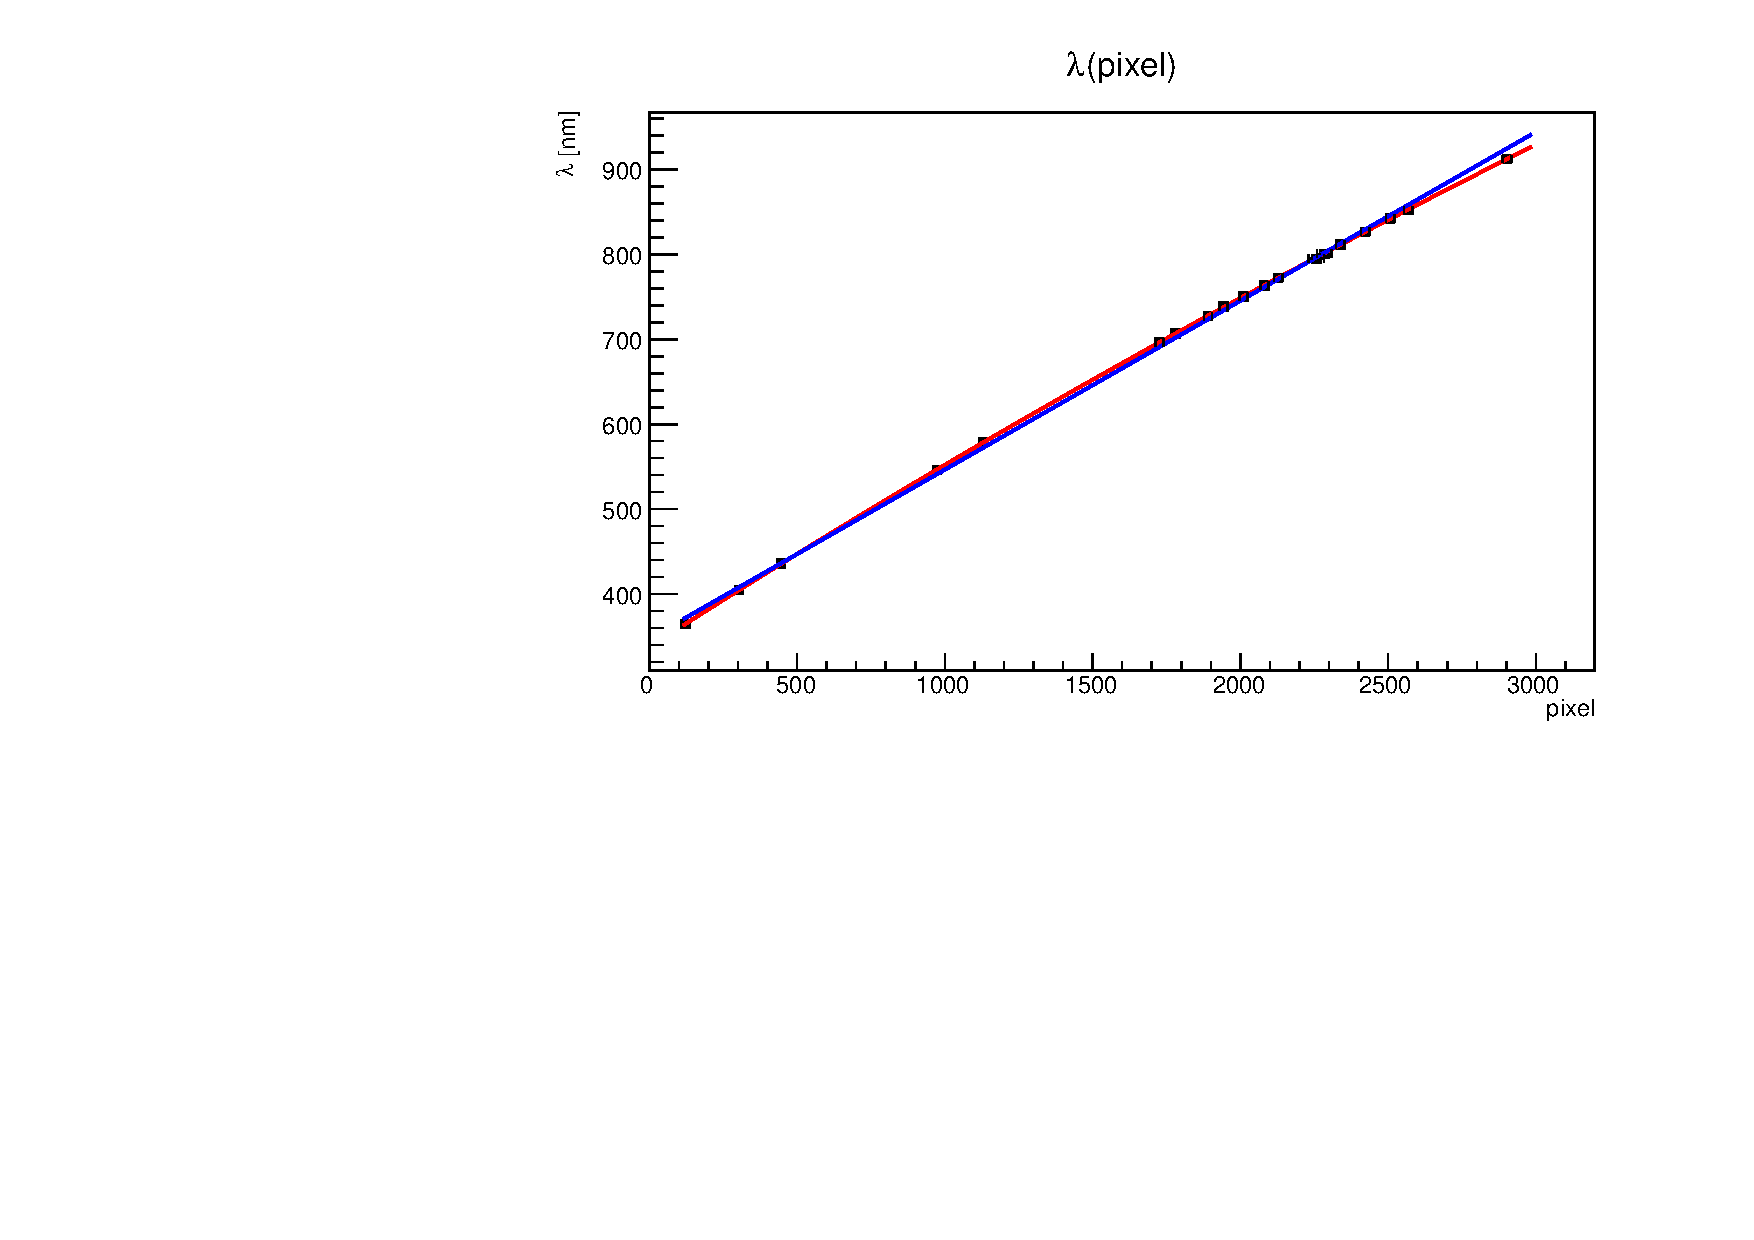
\includegraphics[width=350px]{img/cal_approx.pdf}
\caption{Calibrazione con i dati approssimati.}
\end{center}
\end{figure}
\\Successivamente analizzando i dati acquisiti dello spettro tramite ROOT, si sono svolti fit gaussiani per ogni picco, in modo da stabilire con maggiore precisione i parametri di conversione.\\
Dai risultati estratti si è quindi svolto nuovamente il fit di calibrazione, per utilizzare la miglior legge di conversione disponibile e verificare se l'errore della calibrazione approssimata risultasse significativo.
\begin{figure}[!h]
\centering
    \subfloat[]{{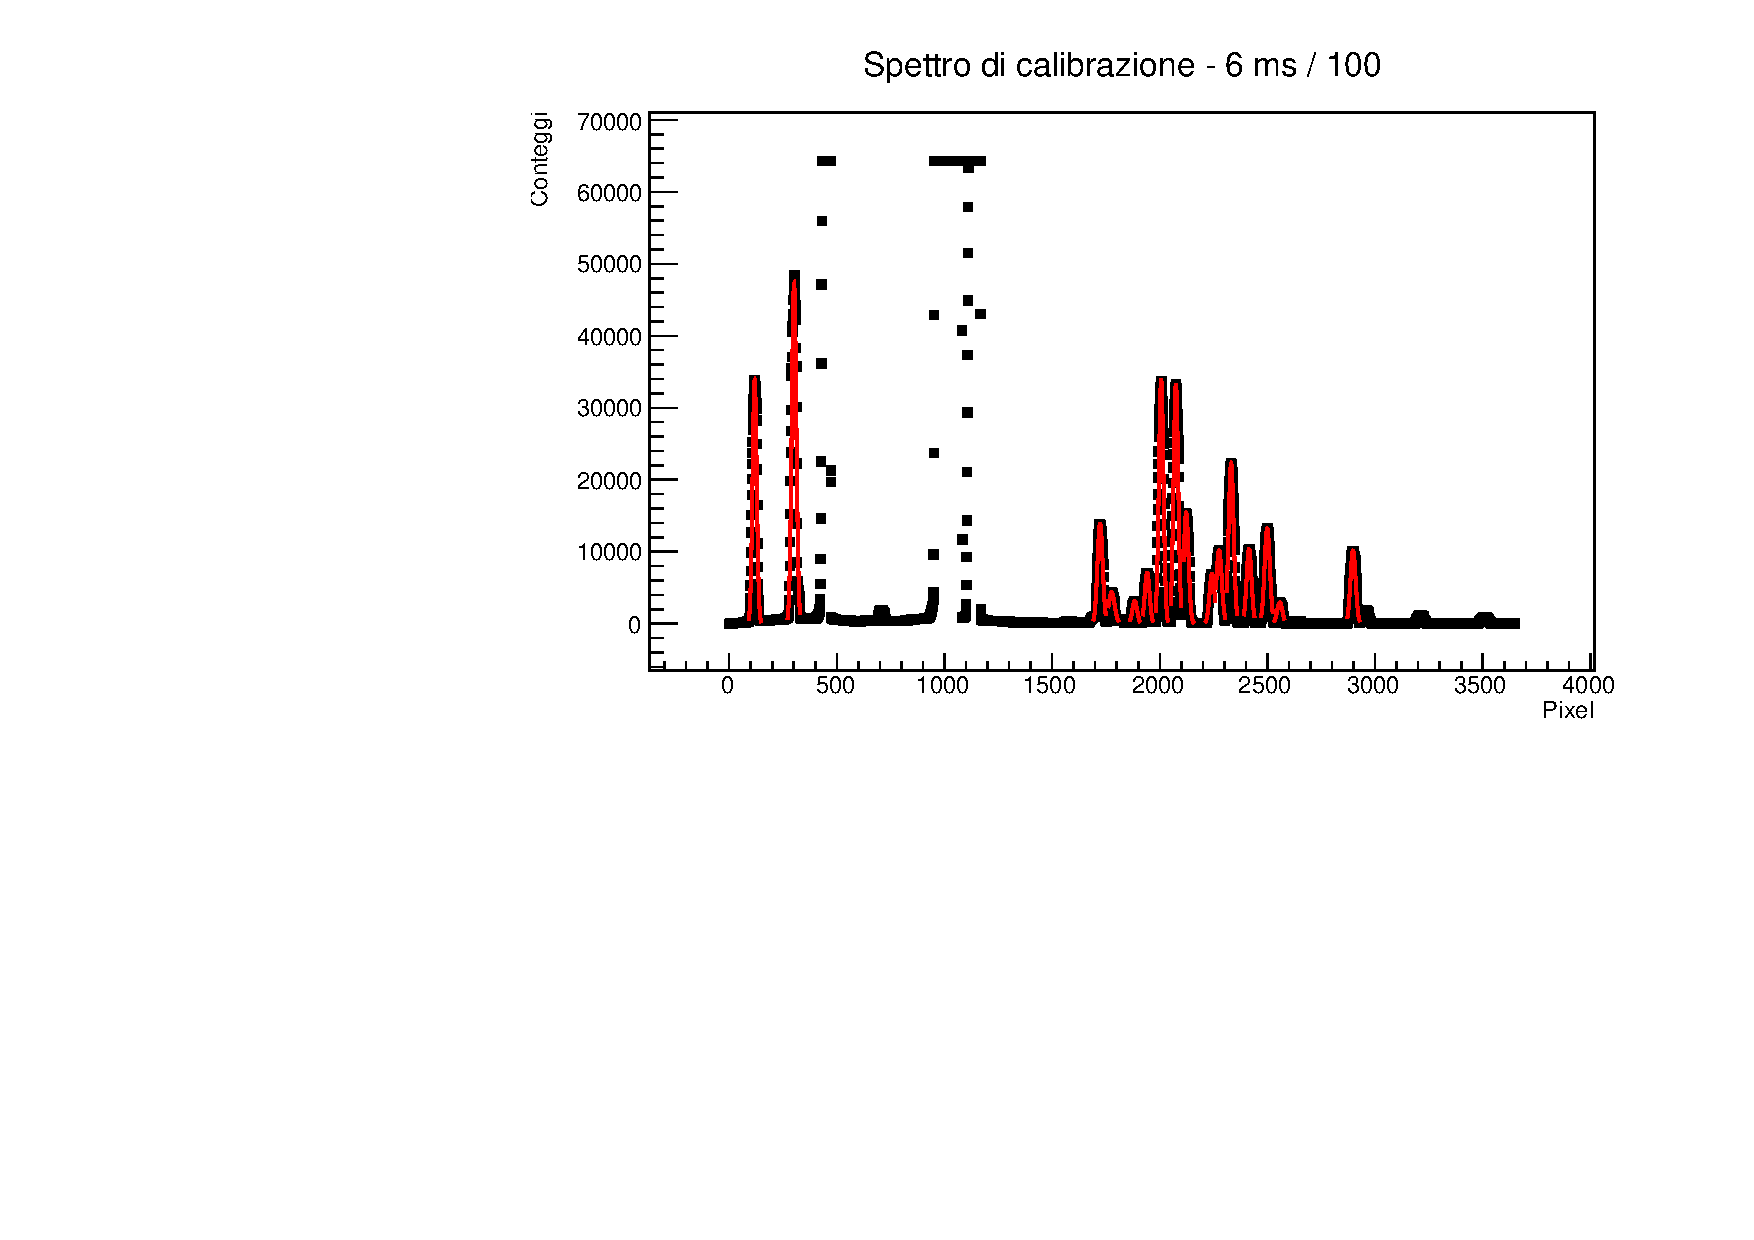
\includegraphics[width=7.9cm]{img/spec_fit.pdf} }}%
    \subfloat[]{{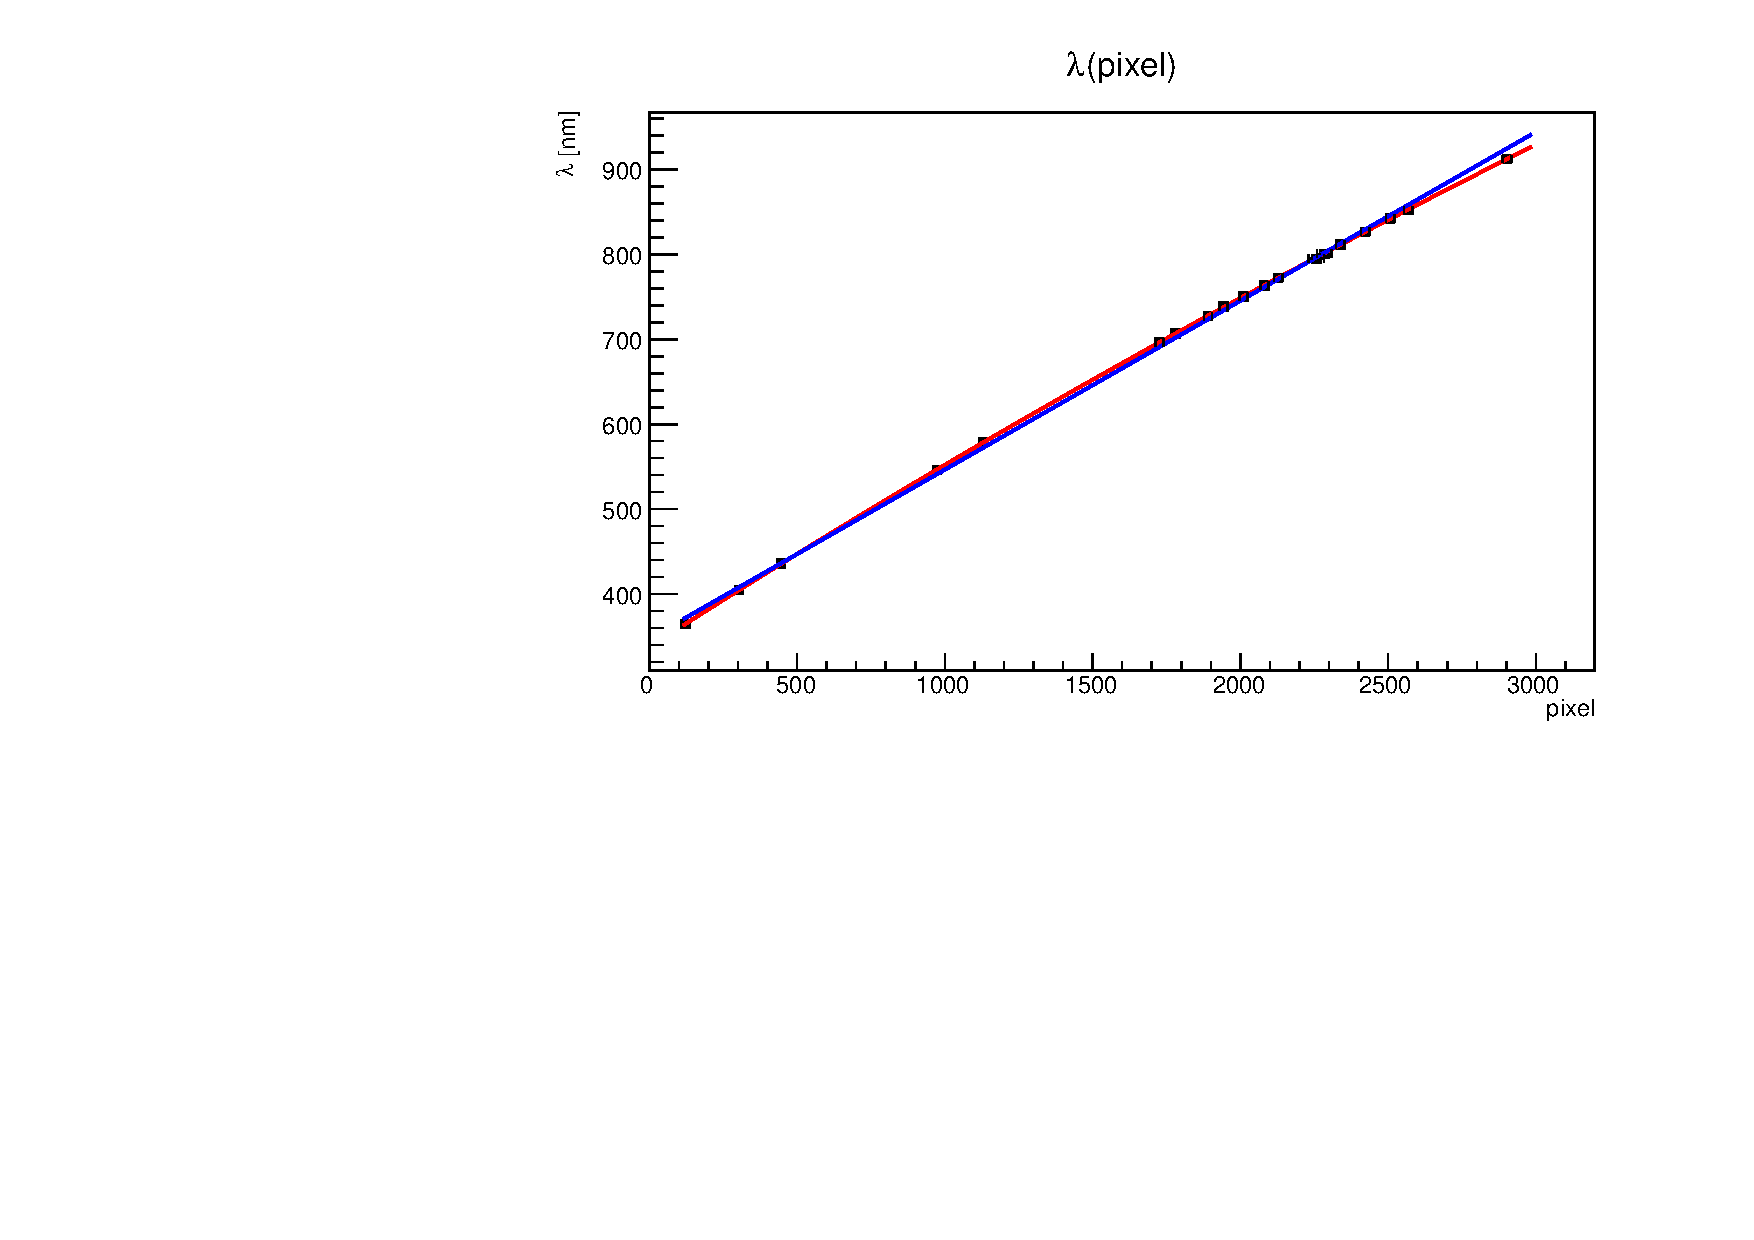
\includegraphics[width=7.9cm]{img/cal_approx.pdf} }}%
\caption{Fit gaussiani dei picchi dello spettro (a) e calibrazione derivata (b).}
\end{figure}
\\
\subsection{Calibrazione del monocromatore interferenziale}
Stabilita la conversione pixel - lunghezza d'onda, si è effettuata la calibrazione del monocromatore lungo lo spettro che successivamente saremo andati ad utilizzare per le misure.
\begin{figure}[h!]
\begin{center}
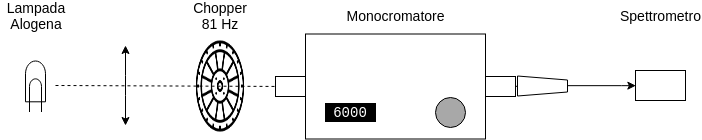
\includegraphics[width=420px]{img/cal_mono.png}
\caption{Setup per la calibrazione del monocromatore.}
\end{center}
\end{figure}
\\Dopo aver allineato il setup sperimentale, si è collegata la fibra ottica al collettore avvitato all'uscita del monocromatore. Accesa la lampada alogena, si sono presi i picchi in uscita per 26 lunghezze d'onda differenti, distanziate fra di loro di 25 unità del monocromatore (1 u $\sim$ 1 nm). Dalle misure prese si sono effettuati fit gaussiani e si è estratta la legge di conversione in lunghezza d'onda.
\begin{figure}[!h]
\centering
    \subfloat[]{{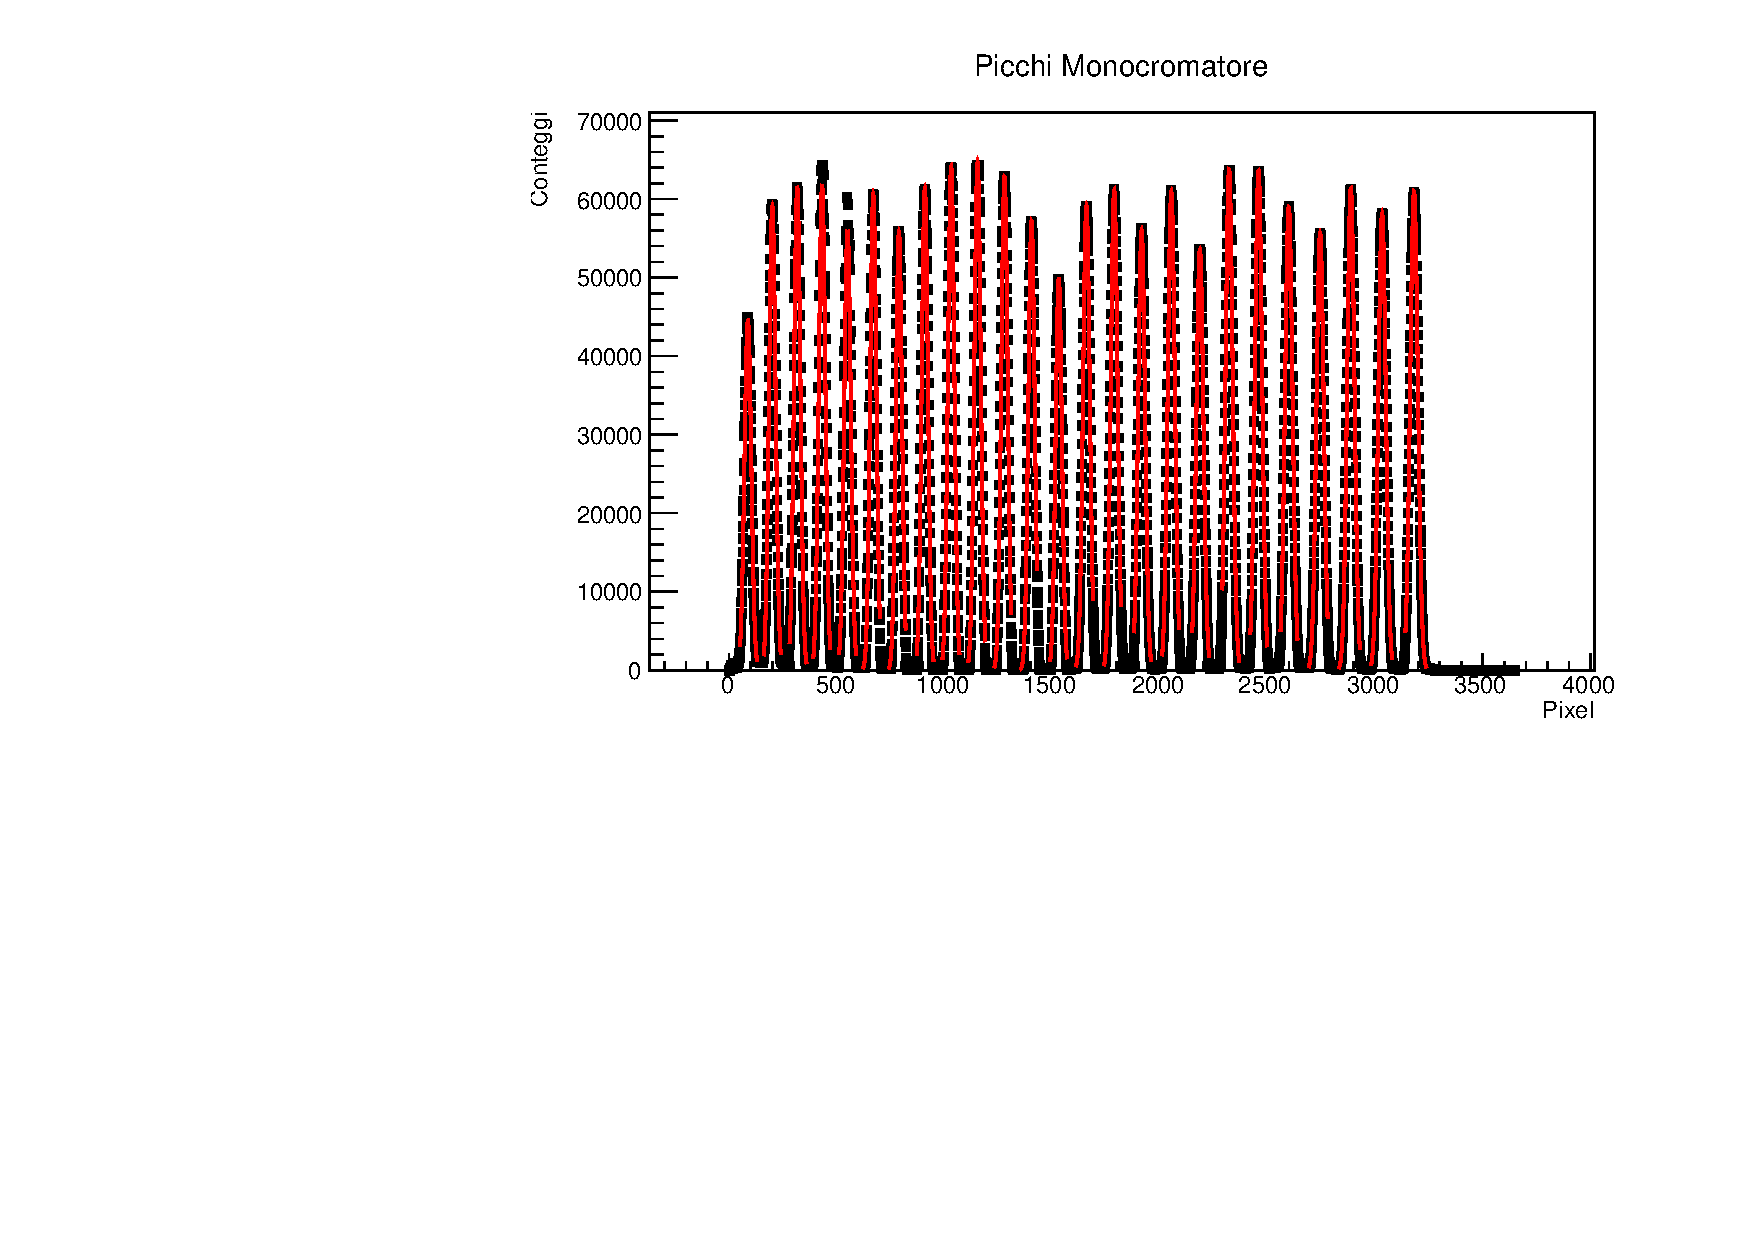
\includegraphics[width=7.9cm]{img/spec_mono.pdf} }}%
    \subfloat[]{{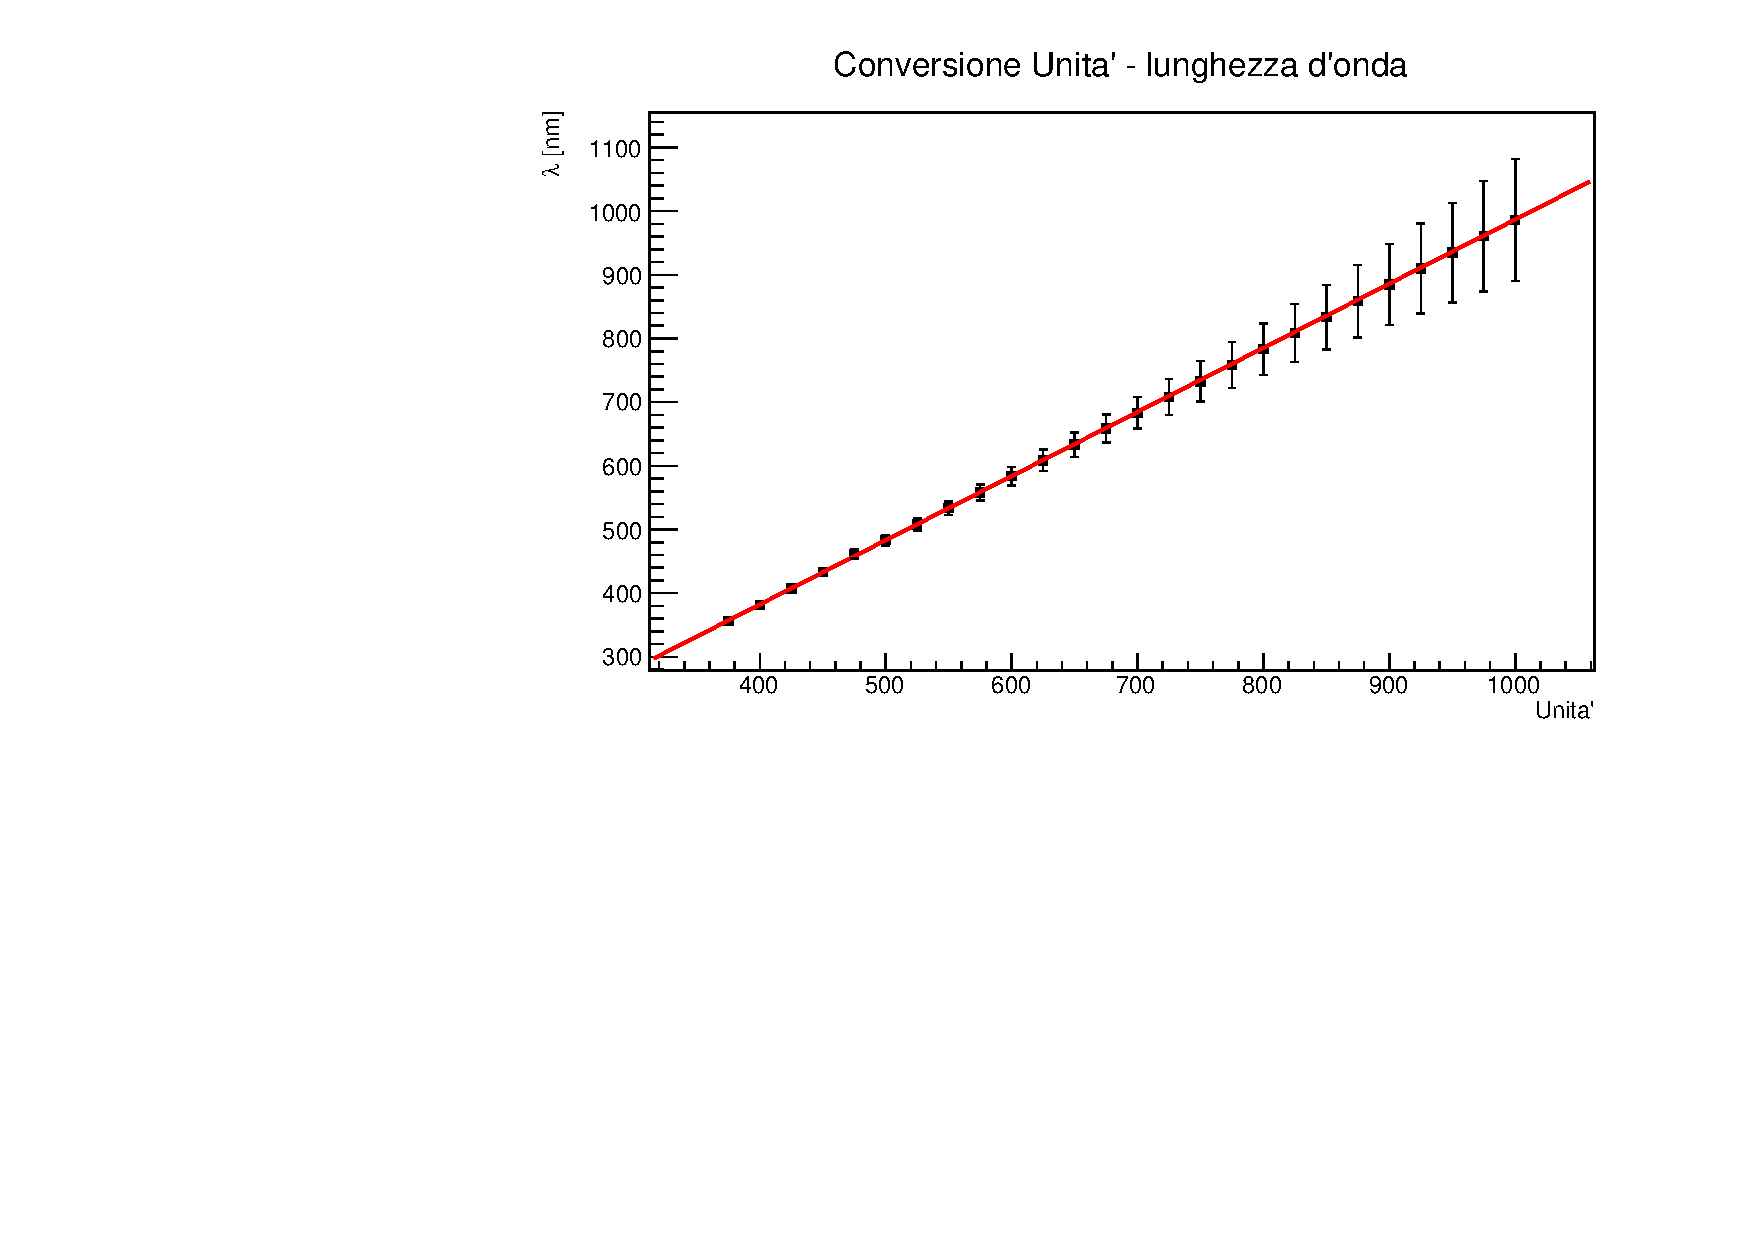
\includegraphics[width=7.9cm]{img/cal_mono.pdf} }}%
\caption{Fit gaussiani dei picchi (a) e calibrazione del monocromatore (b).}
\end{figure}
\\
\section{Misura della fotoconducibilità dei semiconduttori}
Per la misure di fotocorrente e trasmittanza, si è installato un fotodiodo in uscita dal monocromatore,  distanziato in modo da riuscire ad alloggiare i campioni. Prima di effettuare qualunque misura, si è preso lo spettro di riferimento del setup, stabilendo così l'intensità di riferimento.\\
L'inserimento del chopper, il cui scopo è la modulazione del fascio ad una frequenza definita, non è necessario per questa serie di misure, ma ci permette di essere consistenti con le successive che utilizzano l'amplificatore lock-in.
\begin{figure}[h!]
\begin{center}
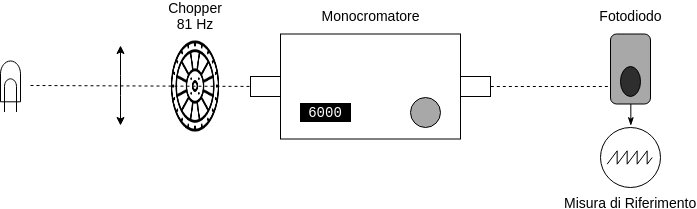
\includegraphics[width=400px]{img/foto_rif.png}
\caption{Setup per la misura dell'intensità di riferimento.}
\end{center}
\end{figure}
\\Per verificare che il vetrino su cui sono applicati i campioni fosse ininfluente, si è ripetuta la misura inserendo un vetrino da 920 $\mu$m all'uscita del monocromatore. Le misure prese sono risultate compatibili, per cui si è determinato che il vetrino non è significativo nel setup.
\subsection{Seleniuro di Gallio - Oscilloscopio}
Inserito il campione di semiconduttore da caratterizzare, si è connessa una tensione di bias di 15 Vdc al campione, mentre l'uscita è collegata all'ingresso dell'oscilloscopio (all'interno del campione è presente un resistore da 1 M$\Omega$ per convertire la fotocorrente in tensione). Per ogni lunghezza d'onda, vengono misurate fotocorrente e intensità della luce trasmessa.
\begin{figure}[h!]
\begin{center}
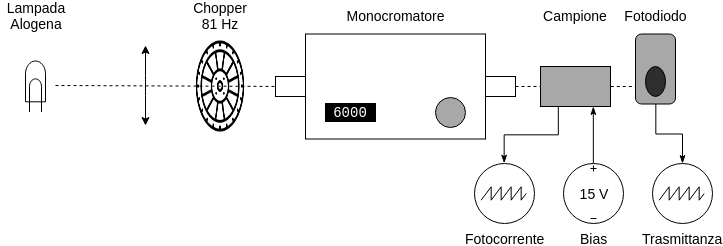
\includegraphics[width=400px]{img/foto_osc.png}
\caption{Setup per la misura della fotocorrente e trasmittanza con l'oscilloscopio.}
\end{center}
\end{figure}

\subsection{Seleniuro di Gallio - Lock-in}
La procedura di misurazione precedente è stata svolta nuovamente utilizzando l'amplificatore lock-in. Questo dispositivo, utilizzando il segnale di riferimento proveniente dal chopper, permette di amplificare il segnale con la medesima frequenza, riducendo così il rumore del resto dello spettro. Questo è necessario in quanto l'oscilloscopio era al limite di risoluzione, in quanto la fotocorrente è molto bassa. Per aumentare ulteriormente la risoluzione della misura, l'uscita dell'amplificatore è stata collegata all'oscilloscopio e misurata utilizzando cursori e funzioni matematiche integrate. L'errore sulle misure di tensione è stato determinato dalla deviazione standard calcolata dall'oscilloscopio su 100 campionamenti.
\begin{figure}[h!]
\begin{center}
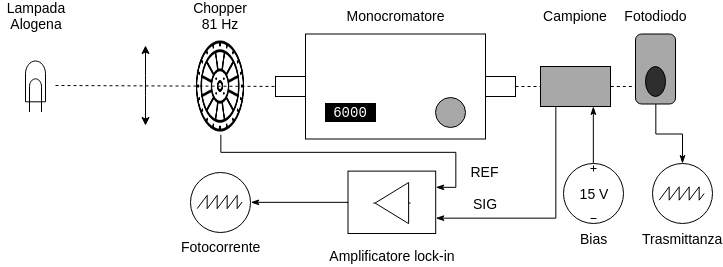
\includegraphics[width=400px]{img/foto_lock.png}
\caption{Setup per la misura della fotocorrente e trasmittanza con l'amplificatore lock-in.}
\end{center}
\end{figure}
\subsection{Arseniuro di Gallio - Lock-in}

\subsection{Campione Sconosciuto - Lock-in}

\appendix
\section{Misura di capacità con l'amplificatore lock-in}
Per impratichirsi con l'amplificatore lock-in, si è voluta misurare una capacità incognita costruendo un partitore di corrente ed eccitandolo con un segnale sinusoidale di 4 Vpp e frequenza variabile. Prima le misure si sono prese con l'oscilloscopio e successivamente utilizzando l'amplificatore. La scelta delle frequenze ha compreso la frequenza di rete e le sue armoniche, in modo da valutare se il lock-in fosse in grado di ridurre il rumore generato.
\section{Misure della trasmittanza con lo spettrometro}
Per la misura della trasmittanza, si sono utilizzate le utility del software dello spettrometro, che disponevano già del calcolo della trasmittanza. Per utilizzarle, si è dovuto prendere uno spettro di riferimento della sorgente luminosa ed uno spettro scuro, comprendente il rumore di fondo. Successivamente attivata la modalità trasmittanza, si è acquisita la risposta dei campioni sullo spettro di riferimento. Per evitare di saturare e avere la miglior risoluzione, si è usata la fibra ottica senza collettore.
\section{Dati e regressioni per la calibrazione}
\subsection{Spettrometro}
\subsection{Monocromatore}

\end{document}
